\section{Multiple object tracking}
\label{sec:mot}
Multiple object tracking (MOT) is to perform simultaneously tracking many objects in a video through locating their positions while maintaining their identities.
MOT task plays an important in many intelligence application, which supplies a helpful tools for complicated analysis works, such as video surveillance, safety monitoring or instance behavior understanding, etc.
Contemporary MOT methods follow the tracking-by-detection paradigm: extract set of detections from consecutive video frames then associate them to construct target tracklets. Therefore, many researches \cite{bergmann2019tracking,zhou2020tracking,bochinski2017high,bewley2016simple} show that if the detectors work well, they provide strong information cues to associate objects, hence boost the tracking performance. 
In general, tracking-by-detection MOT algorithms share parts of the following steps:
\begin{itemize}
    \item \textbf{Detection stage}: an object detectors is utilized to locate all potential objects which could be appearance of our concerned targets.
    \item \textbf{Feature Extraction stage}: apparent or motion feature represents each detected objects is extracted for further comparison.
    \item \textbf{Similarity Measure stage}: Representation features are used to compute similarity/distance score between detected tracks so far and new detections.
    \item \textbf{Association stage}: assign target ID to detected objects based on matching scores from previous steps.
\end{itemize}
\begin{figure}[t!]
    \centering
    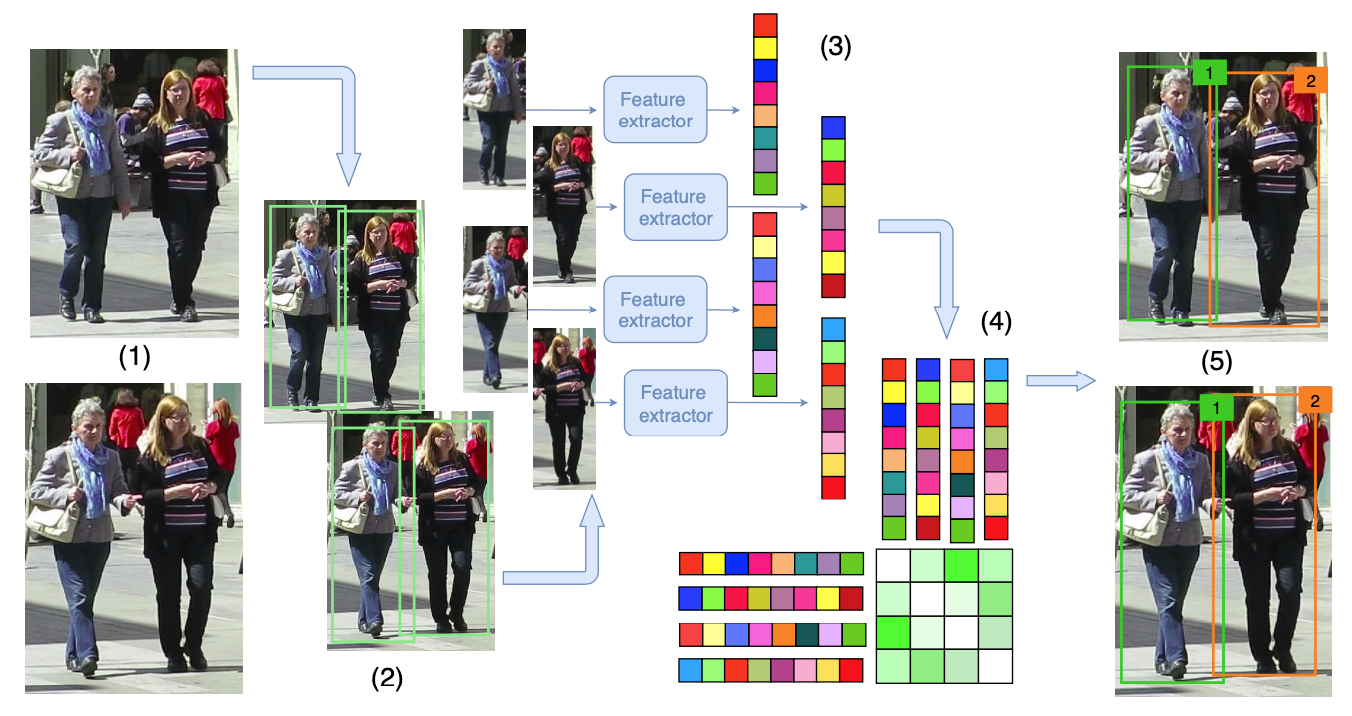
\includegraphics[width=0.9\textwidth]{resources/images/MOT_overview.png}
    \caption{An overview of common MOT algorithms workflow. For each consecutive frames (1), the algorithm first detect all potential objects (2), then extract their representation features (3) and adopt pair-wise comparison (4) to associate most similar objects with the same ID (5). \cite{ciaparrone2020deep}}
    \label{fig:MOT_overview}
\end{figure}
Figure \ref{fig:MOT_overview} shows the step-by-step procedure of common MOT approaches.\\
Common algorithms solved MOT problem can be divided into two main groups: offline and online methods. 
Offline learning (batch based tracking) \cite{rezatofighi2015joint,kim2015multiple} assumes that the system has seen the whole video before start processing. 
Online learning approaches are only allowed to process and update tracking results frame by frame. Due to the efficiency and practicality, online and realtime algorithms achieves more attention. Many works \cite{pang2021quasi, zhou2020tracking, bergmann2019tracking, wojke2017simple} have been proposed to explore this type of learning and achieve potential results on benchmark settings and in practical situations. 
% In the scope of this project, we modified the DeepSORT \cite{wojke2017simple} method as a submodule for our retrieval system.

\subsection{SORT algorithm}
\label{sec:sort}
We first briefly discuss one of the most popular online tracking method, which successfully leverage ConvNet for detection step to achieve state-of-the-art result at the time it proposed, the Simple Online and Realtime Tracking (SORT) \cite{bewley2016simple} algorithm.
The important features of SORT compose: target detections based on Faster-RCNN \cite{NIPS2015_14bfa6bb} architecture, the use of Kalman filter \cite{kalman1960new} to forecast target positions at each time step and Hungarian algorithm \cite{kuhn1955hungarian} for the similarity matching step between current tracks and new detected objects. These modules help to achieve potential accuracy while greatly improves the speed of tracking multiple targets at the same time. \\
\begin{figure}[t!]
    \centering
    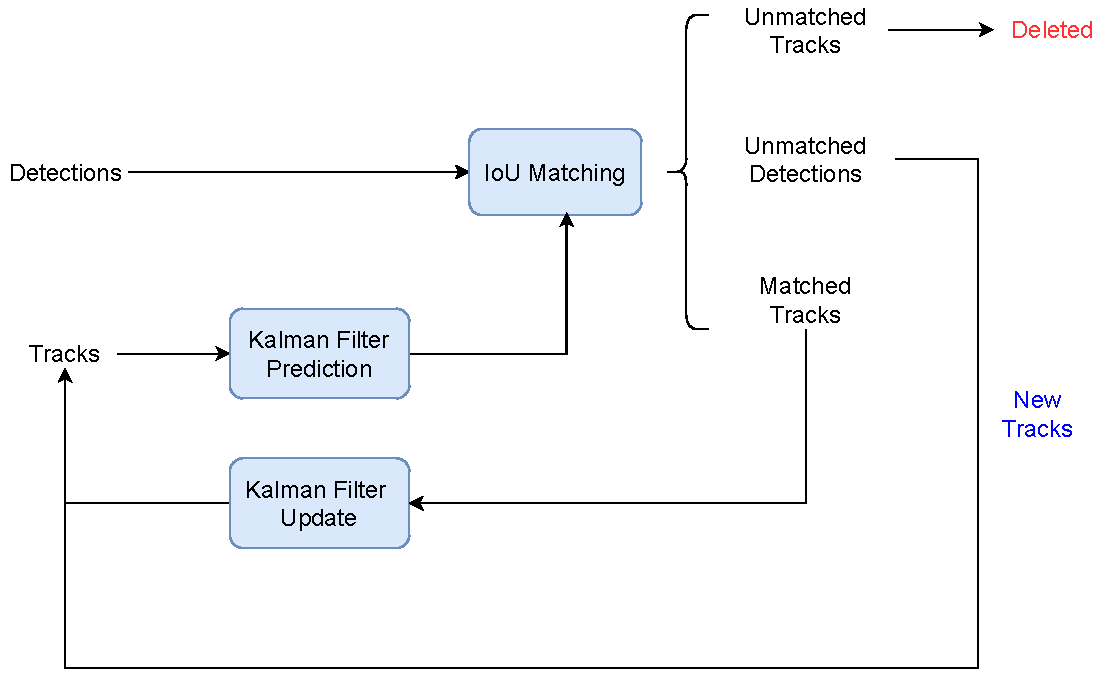
\includegraphics[width=0.9\textwidth]{resources/images/SORT.pdf}
    \caption{SORT algorithm's processing flow.}
    \label{fig:SORT_overview}
\end{figure}
At each time step $t$-th, let $T$ denotes list of tracks we have successfully associate so far, the SORT algorithm works as follow:
\begin{itemize}
    \item \textbf{Detection stage}. \\
    The method utilizes an detector model to detect all potential objects current frame. Suppose that we have $N$ boxes at this frame.
    
    \item \textbf{Kalman Filter prediction stage}. \\
    For each track in $T$, Kalman Filter uses those movement states from previous frames to predicts the target position and speed at current frame. 
    The SORT algorithm works with assumptions that all targets have linear constant velocity and their movements are independent with the others. Hence, a state of target object at a specific time step is implemented as follow.
    \begin{align}
        \label{eqn:sort_kf}
        \mathbf{x} = [u,v,s,r,\dot{u},\dot{v},\dot{s}]
    \end{align}
    where $u, v$ represents the horizontal and vertical coordinate of the target center respectively. While $s$ is the bounding box area and $r$ is the corresponding aspect ratio. $\dot{u},\dot{v},\dot{s}$ denotes the velocity of those values at current time $t$.
    \item \textbf{IOU matching stage}. \\
    Those predicted states at current frame are used to compute a similarity matrix between $T$ tracks and $N$ detected boxes based on IoU score, result in a similar matrix of size $[N \times T]$. Hungary algorithm is then applied on this matrix to produce best matching detection for each track.
    \item \textbf{Confirmation stage}. \\
    Those with similarity score is higher than a threshold are considered as \textit{matched tracks}. Otherwise, tracks with small similarity are seen as disappear from current frame and removed from the system memory. Detections that are not currently matched with any tracks are used to initialize as \textit{new tracks} and saved to the memory.
    \item \textbf{Kalman Filter Update stage}. \\
    The predicted and observed values of matched tracks are linearly weighted to update the current state representation.
\end{itemize}
Figure \ref{fig:SORT_overview} illustrates the workflow of SORT algorithm at each frame.\\
However, SORT algorithm still have some drawbacks when running on those hard cases. The first problem is with the linear assumption of Kalman Filter framework, in practice, the targets rarely move with constant velocity.
And second, ID switches is the biggest drawback of SORT. The association between detections and tracks is simply based on IoU measure, which indicates that the algorithm only cares about the object shape, this causes the phenomenon that the number of ID switches of an object is extremely large when the object is obscured or when the trajectory overlaps with the others.

\subsection{Deep SORT algorithm}
\label{sec:deep_sort}
In this section, we consider another tracking approach that built as an extension to SORT algorithm, Deep SORT \cite{wojke2017simple}. To address the disadvantages of SORT, Deep SORT utilize deep learning network to extract features of detected objects to enhance the data association process. Furthermore, a matching cascade strategy with a new confirmation strategy is proposed to handle the problem of occlusion tracks. These improvements are shown in figure ... .
As compare to figure(SORT), Deep SORT adds a \textit{Matching Cascade} module and a new trajectory confirmation strategy to the original SORT algorithm. \\
To handle the occlusion problem, Deep SORT manages life-cycle of each archived track based on a state variable with three values (\textit{tentative}/\textit{unconfirmed}, \textit{confirmed}, \textit{deleted}). 
\begin{itemize}
    \item Each new track is initialized as \textit{unconfirmed}. Through the filtering process, if the track is not removed in the next three frames, it becomes \textit{confirmed} track, and will stay filtered for the next $max\_age$ frames.
    \item Otherwise, if the track is lost when less then 3 frames are reached, it will be deleted.
\end{itemize}

\begin{figure}[t!]
    \centering
    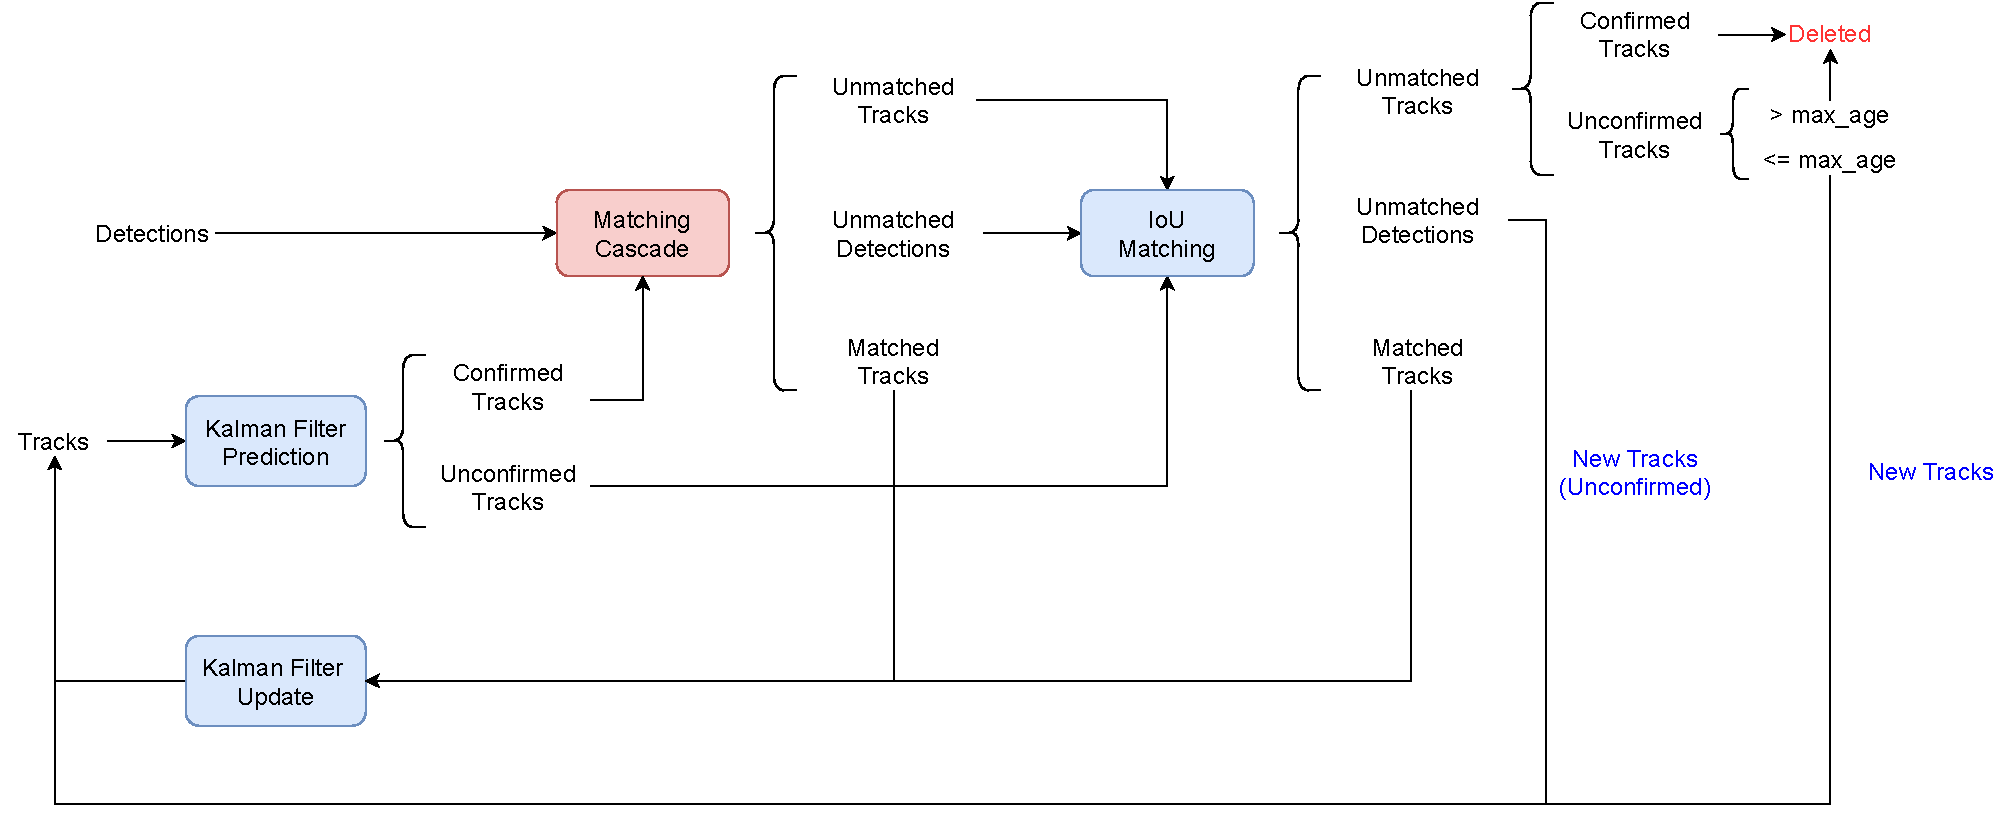
\includegraphics[width=\textwidth]{resources/images/DeepSORT.pdf}
    \caption{Deep SORT algorithm's processing flow.}
    \label{fig:DeepSORT_overview}
\end{figure}

The details of each stage in Deep SORT process are described as follows (shown in figure \ref{fig:DeepSORT_overview}).
\begin{itemize}
    \item \textbf{Detection stage}. \\
    Same as SORT algorithm, Deep SORT use an object detector to detect all potential boxes at current frame.
    \item \textbf{Kalman Fitler Prediction and Update stage}. \\
    Same as SORT algorithm, predict next representation to perform prediction and update current state if finding new detection for each track.
    \item \textbf{Filter Layer 1: Matching Cascade}. \\
    The Matching Cascade takes in a list of archived tracks $T$ and assign them to best matching objects from $N$ detections at current frame. Different from the original SORT, Deep SORT integrates both motion feature and appearance feature to measure the similarity. 
    Motion feature is modelled the same way as the SORT algorithm (\ref{eqn:sort_kf}), while the appearance descriptor is extracted from pretrained CNN-based network trained with re-identification settings. 
    In general, the similarity measure between track $i$ and object $j$ is formulated as follow
    \begin{align}
        \label{eqn:deepsort_score}
        c_{i,j} = \lambda d_{motion}(i, j) + (1-\lambda) d_{appearance}(i, j)
    \end{align}
    Where Mahalanobis distance is used to measure motion uncertainty $d_{motion}$ and Cosine distance is used for appearance measure $d_{appearance}$. \\
    With the computed similarity matrix, Deep SORT then applies multi-step thresholding on archived tracks based on their ages, and finally produce list of matched tracks, unmatched detections and unmatched tracks.
    \item \textbf{Filter Layer 2: IoU Matching}. \\
    This filter apply IoU association with the same strategy as SORT on unlinked tracks and detections from previous layer and archived unconfirmed tracks. 
    \item \textbf{Confirmation stage}. \\
    After the two layers of filtering, unconfirmed tracks that still not match with any detections of confirmed tracks which have stayed too long in the memory (larger than $max\_age$) are removed. Unmatched detections are used to create new tracks and the procedure starts over with the next frame.
\end{itemize}
In the scope of this project, we modified the DeepSORT algorithm \cite{wojke2017simple} to utilize as a sub-module that captures the relationships between target object and neighboring vehicles.
